\section{Cell Movement}

% 5 marks for definitions of distributions and reasons behind the choice of distribution

The random movement of cells should be modelled using a probability distribution

There are several probability distributions that can be classified as discrete or continuous, we will analyse uniform, bernoulli and beta.

The uniform distribution is usually regarded as a continuous distribution but can also be used to model discrete variables. 

Area under the graph is one

\[ f(x) =\begin{cases}a & \text{if } x = 1\\b & \text{if } x = 0\end{cases}\]

\[ f(x) =\begin{cases}1 & \text{for } 0  \leq x  \leq  1\\0 & \text{otherwise}\end{cases}\]

Uniform distribution
Definition of distributions
Uniform distributions
Bernoulli Distribution

Bias introduced with different distributions


When all directions are equally probable a uniform distribution could be used.

If a Bernoulli distribution was selected, it would introduce a bias to the direction of movement
This could be desired in a complex model where factors such as surface tension affect the direction of movement

% how random numbers are actually generated in rust

% complexity of the different movements
%  all o^n but increase the multiplier of n

% Movement directions

% 'Complexity of direction methods'

\clearpage

Both directions have bias

Square goes to right, diagonal goes down 

This is because it is a single step run, the number generation is random, hence direction is random

100 steps, diagonal moves further than square

\begin{figure}[ht]
    \centering
    \begin{subfigure}{0.45\textwidth}
    	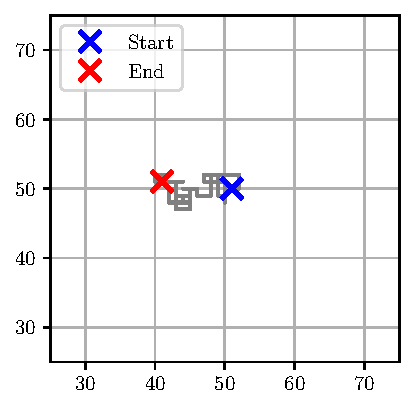
\includegraphics[width=\textwidth]{task1-1}
    	\caption[Square]{Square}
    	\label{fig:task1-1}
    \end{subfigure}
    \begin{subfigure}{0.45\textwidth}
    	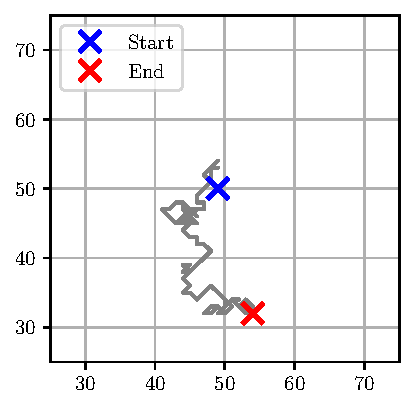
\includegraphics[width=\textwidth]{task1-2}
    	\caption[Diagonal]{Diagonal}
    	\label{fig:task1-2}
	\end{subfigure}
	\caption[Cell movement plots]{Cell movement plots}
    \label{fig:task1}
\end{figure}

\clearpage

By mapping the visited cells, we can see the difference in the movement of the cells across thousands of steps to validate the evenness of the uniform distribution.

Select random start and end points using a uniform distribution, iterate until end point is reached

Small hotspots, but overall even distribution

With more iterations, the distribution will be more even

Validates the uniform distribution of both the square and diagonal movements

And validates the uniform distribution of the random start and end points

\begin{figure}[ht]
    \centering
    \begin{subfigure}{0.45\textwidth}
        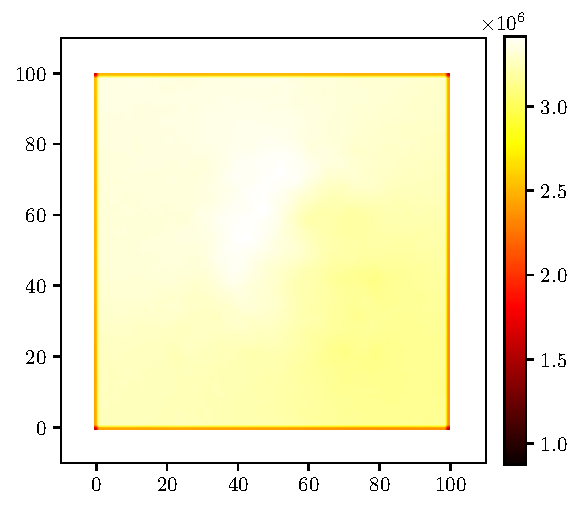
\includegraphics[width=\textwidth]{task1-visited-square}
        \caption[Square]{Square}
        \label{fig:task1-visited-square}
    \end{subfigure}
    \begin{subfigure}{0.45\textwidth}
        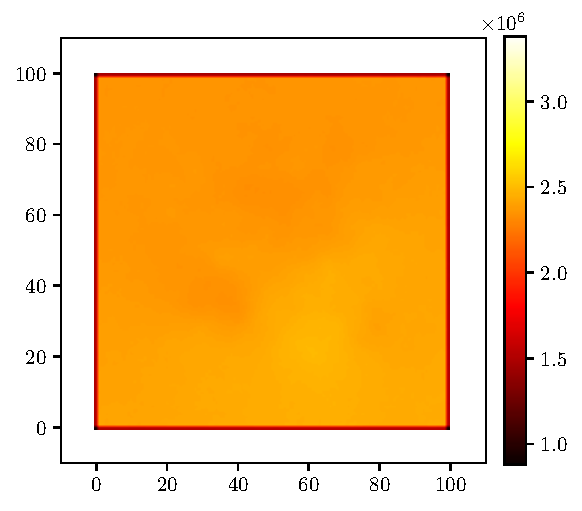
\includegraphics[width=\textwidth]{task1-visited-diagonal}
        \caption[Diagonal]{Diagonal}
        \label{fig:task1-visited-diagonal}
    \end{subfigure}
    \caption[Visited cells simulation heatmap]{Visited cells simulation heatmap}
    \label{fig:task1-visited}
\end{figure}

There is a significant difference in the number of visited cells between the square and diagonal movements.

This is because the diagonal movement can move further in a single step than the square movement.

The square can perform one step to the left, right, up or down.

The diagonal can perform one step to the left, right, up, down, up-left, up-right, down-left or down-right.
Any diagonal movement is equivalent to two square movements.

Hence square movement is on average $(1 \times 4) / 4 = 1$ steps

The diagonal movement is on average $(\sqrt{2} \times 4 + 1 \times 4) / 8 = 1.2071$ steps

Square is factor of $1 / 1.2071 = 0.8284$ compared to diagonal

Hence in the scene of moving from one point to another, the diagonal movement is more efficient than the square movement.

However, this is different from computational complexity, where the square movement is more efficient than the diagonal movement.

% TODO - explain the computational complexity of the different movements

% \begin{figure}[ht]
%     \centering
%     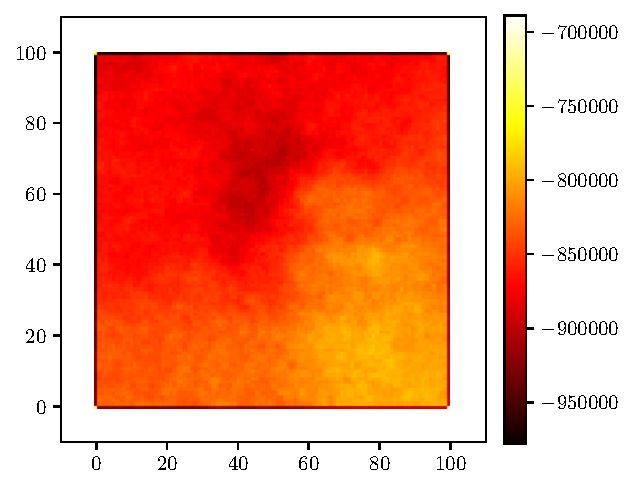
\includegraphics[width=0.45\textwidth]{task1-visited-diff}
%     \caption[Difference in visited cells between square and diagonal simulation heatmap]{Difference in visited cells between square and diagonal simulation heatmap}
%     \label{fig:task1-visited-diff}
% \end{figure}

\clearpage

\begin{figure}[ht]
    \centering
    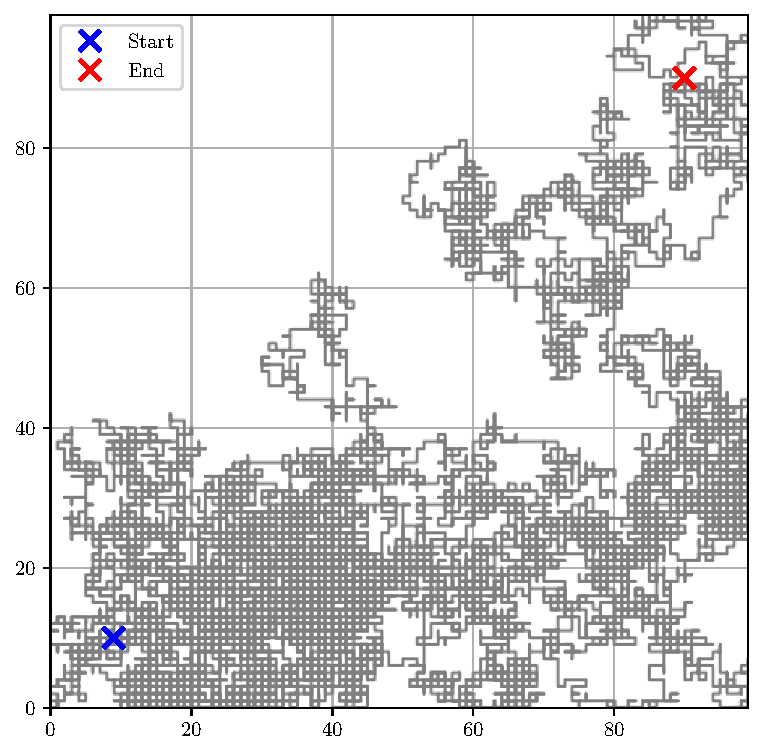
\includegraphics[width=10cm]{task1-1-fill}
    \caption[Square cell movement plot with fill]{Square cell movement plot with fill}
    \label{fig:task1-1-fill}
\end{figure}

\begin{figure}[ht]
    \centering
    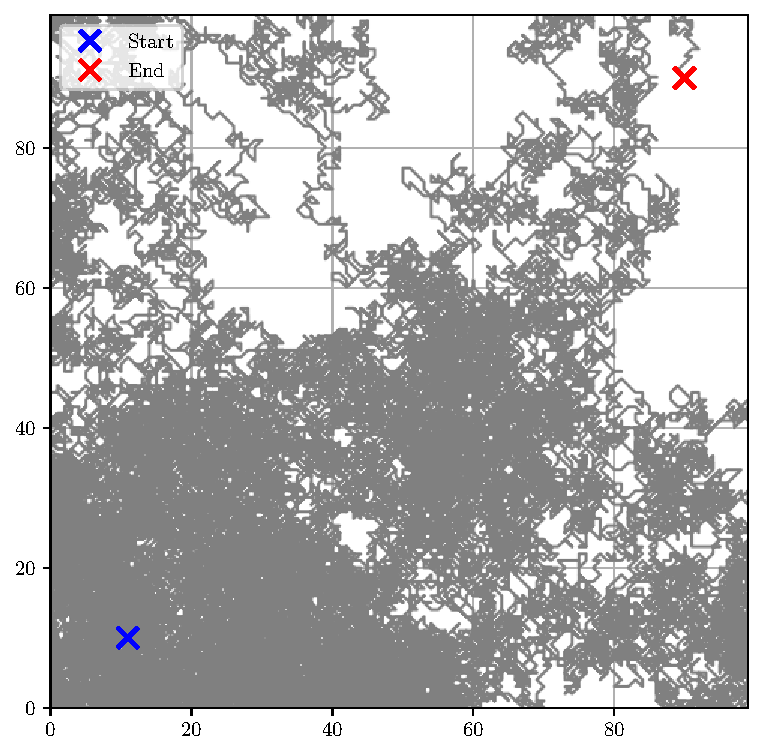
\includegraphics[width=10cm]{task1-2-fill}
    \caption[Diagonal cell movement plot with fill]{Diagonal cell movement plot with fill}
    \label{fig:task1-2-fill}
\end{figure}

\clearpage

Measure the computational complexity of the different movements.

\begin{figure}[ht]
    \centering
    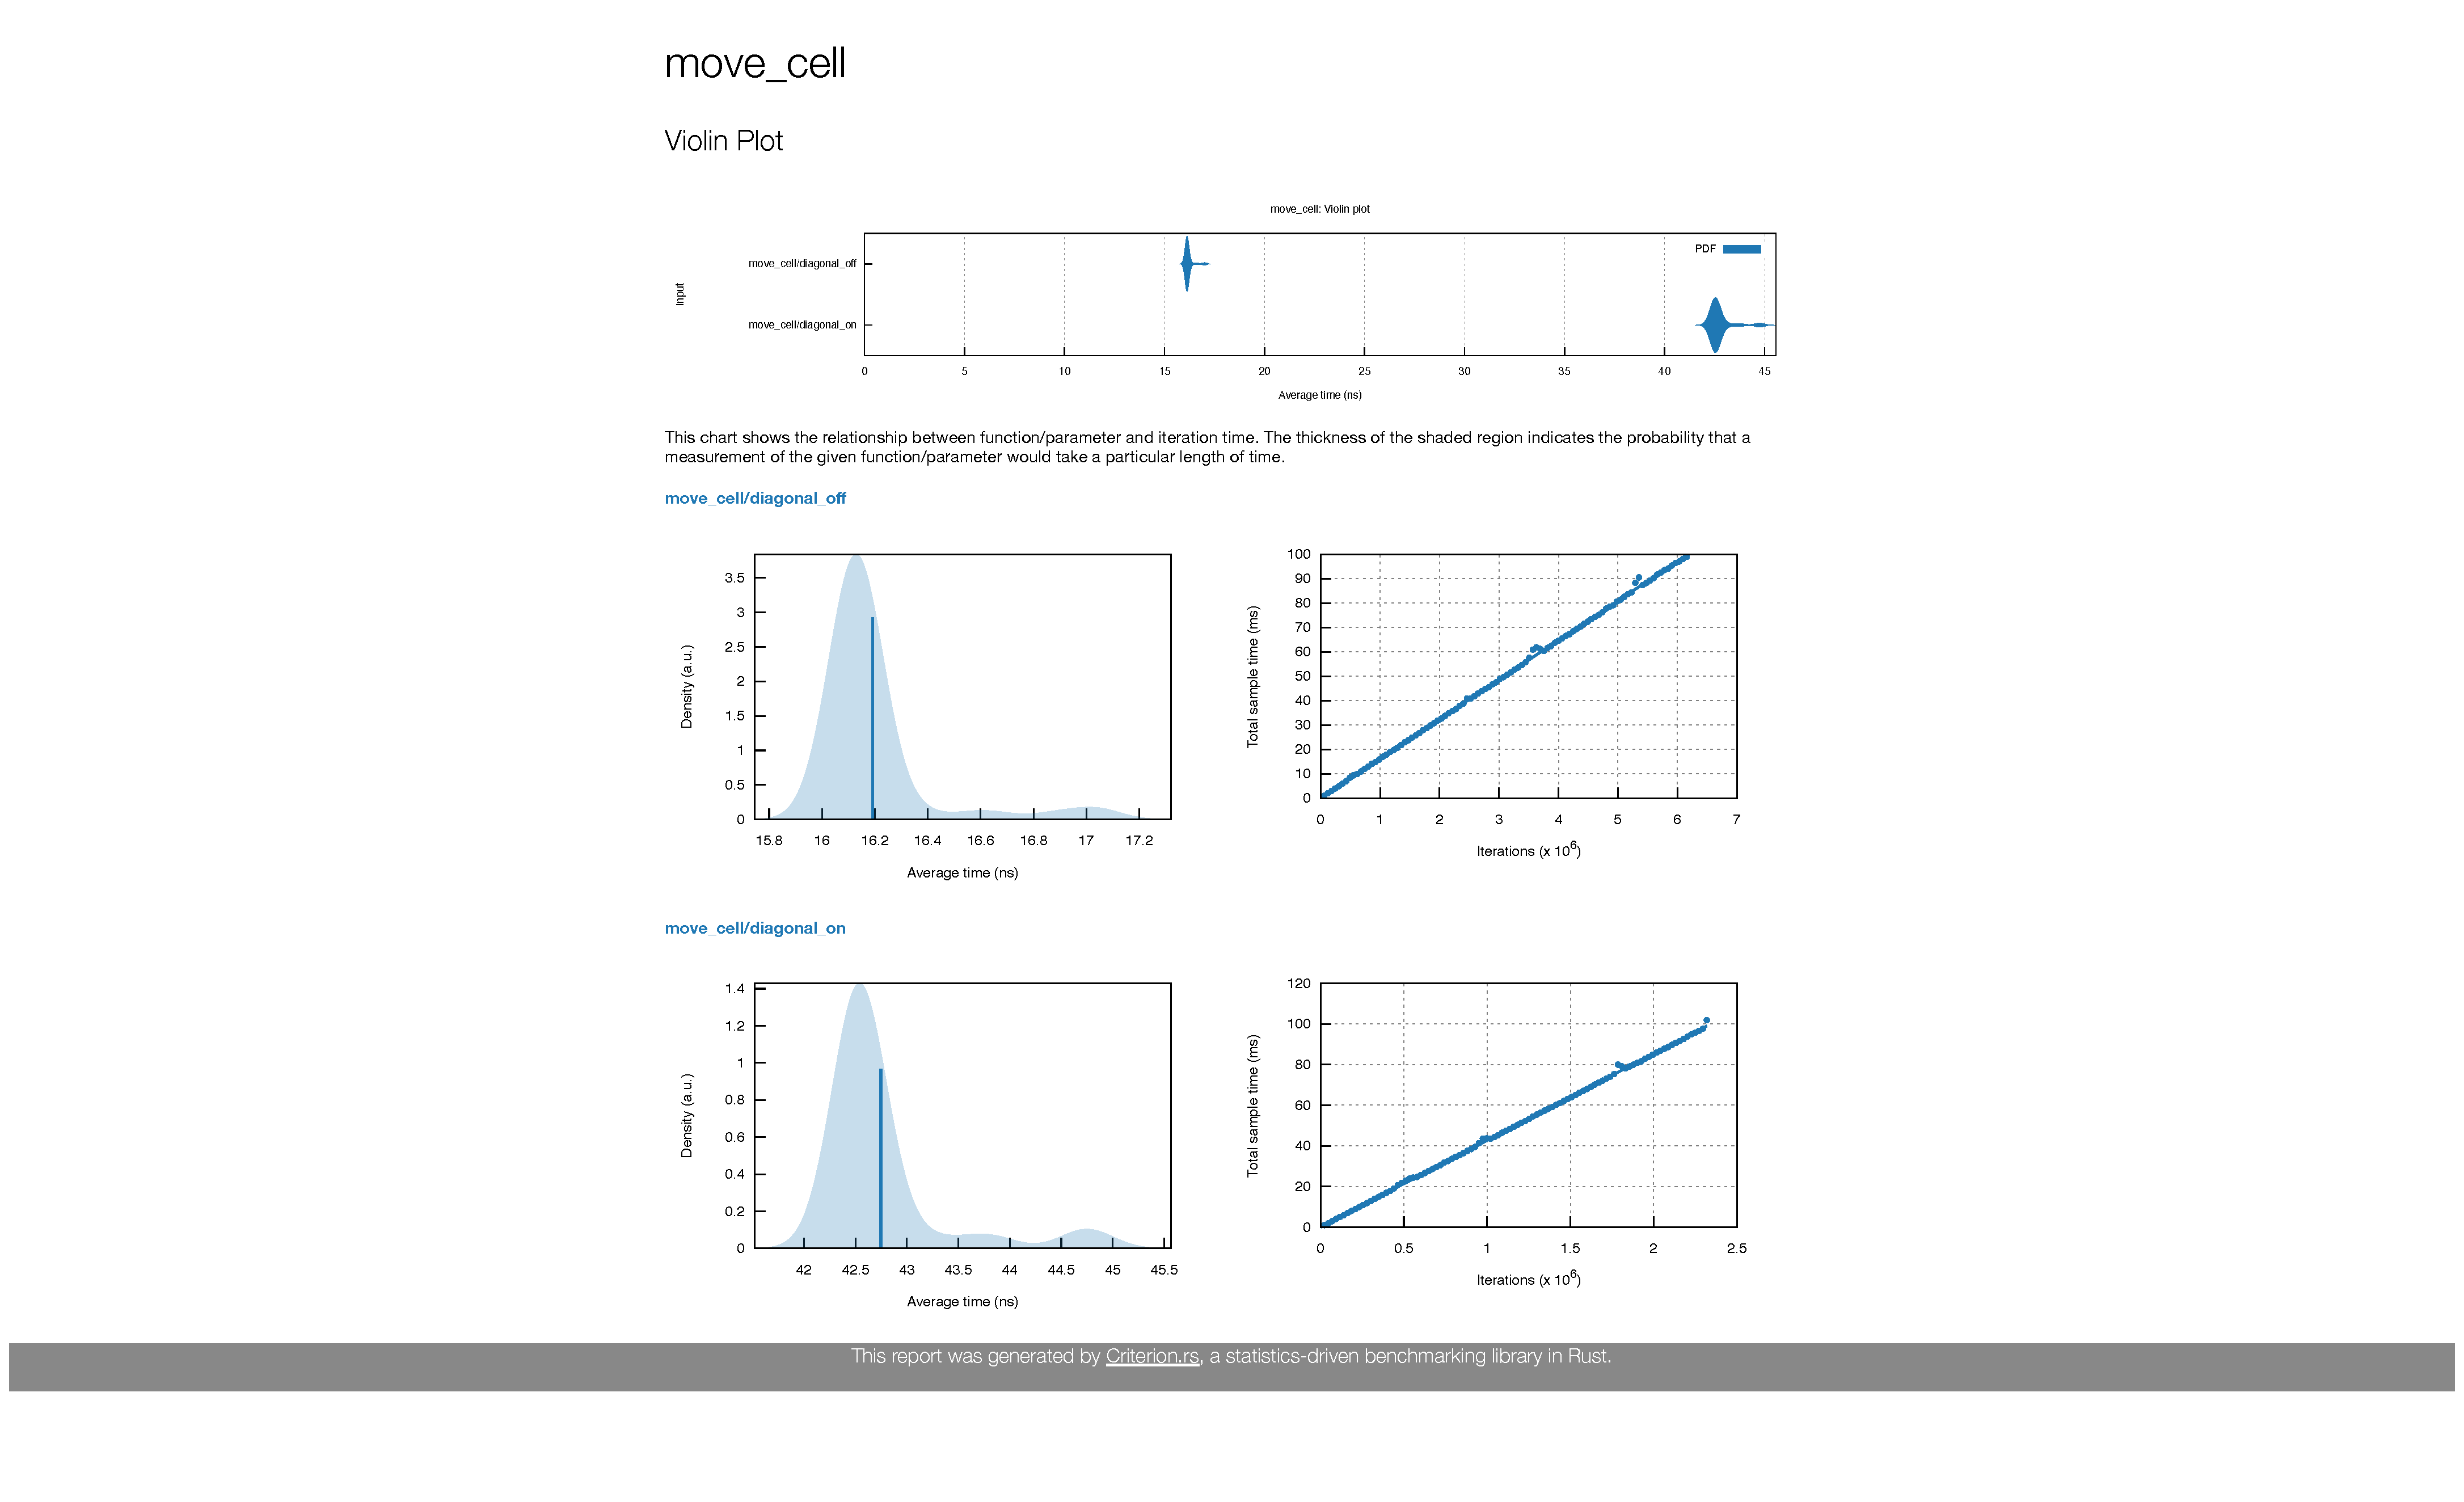
\includegraphics[width=14cm]{move-cell-criterion}
    \caption[Cell movement criterion]{Cell movement criterion}
    \label{fig:move-cell-criterion}
\end{figure}

Square takes 16.2ns

Diagonal takes 42.7ns

This is a ratio of 0.3794

Diagonal movement is more computationally complex than square movement.

This is because the diagonal movement requires more checks to ensure the cell does not move off the grid.

The act of generating a random number is the same for both movements as a single random number is generated to determine the direction of movement, regardless of the movement method.

\clearpage

By selecting a random start and end point, we can compare the number of steps taken by the square and diagonal movements.

If this movement simulation is performed multiple times, the average number of steps taken by the square and diagonal movements can be compared.

Given enough iterations, the average should stabilise and the difference in the number of steps taken by the square and diagonal movements can be calculated.

Non Diagonal - (74, 67) - (55, 40) - 32534.4086

Diagonal - (74, 67) - (55, 40) - 23247.6747

\begin{figure}[ht]
    \centering
    \begin{subfigure}{\textwidth}
        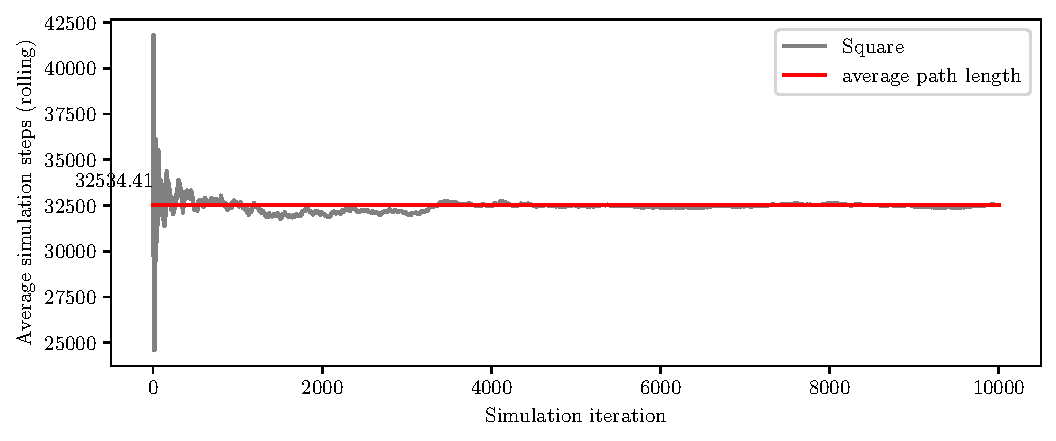
\includegraphics[width=\textwidth]{task1-compare-square-roll}
        \caption[Square]{Square}
        \label{fig:task1-compare-square-roll}
    \end{subfigure}

    \begin{subfigure}{\textwidth}
        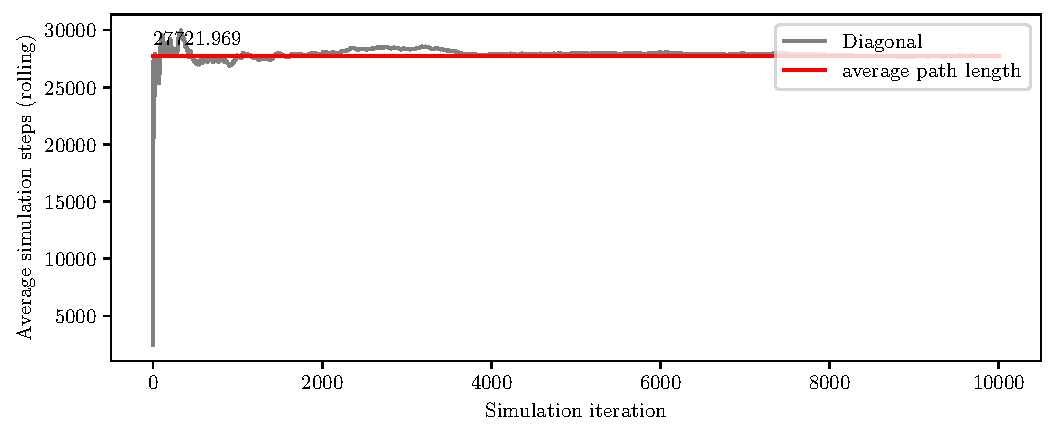
\includegraphics[width=\textwidth]{task1-compare-diagonal-roll}
        \caption[Diagonal]{Diagonal}
        \label{fig:task1-compare-diagonal-roll}
    \end{subfigure}

    \caption[Comparison of square and diagonal simulation steps]{Comparison of square and diagonal simulation steps}
    \label{fig:task1-compare-roll}
\end{figure}

Plotting on to the same graph...

\begin{figure}[ht]
    \centering
    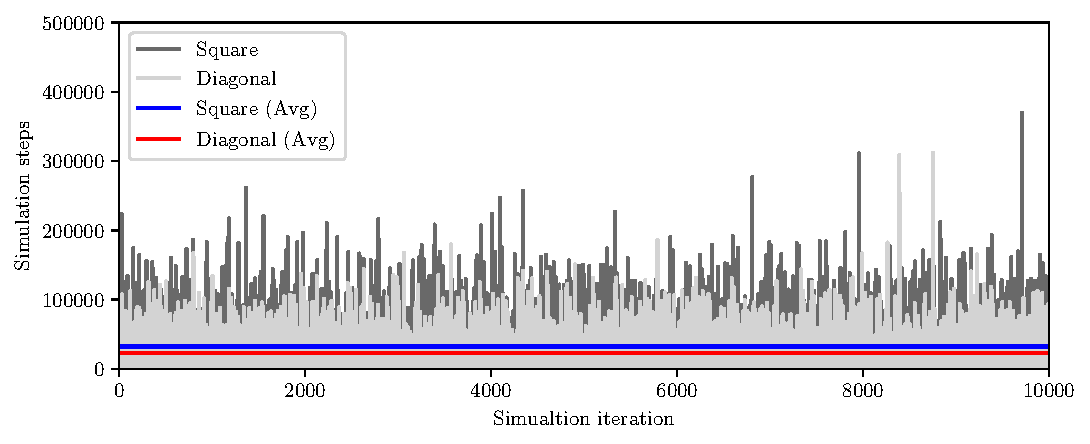
\includegraphics[width=14cm]{task1-compare-single}
    \caption[Comparison of square and diagonal simulation steps]{Comparison of square and diagonal simulation steps}
    \label{fig:task1-compare-single}
\end{figure}

\clearpage

Taking the same process and applying it to multiple different start and end points 

Measure the average number of steps taken by the square and diagonal movements for a given distance between the start and end points.

Also measure the average time taken by the movements.

% By plotting the average number of steps against the distance between the start and end points...

% we can establish an average difference in the number of steps taken by the square and diagonal movements.


\begin{figure}[ht]
    \centering
    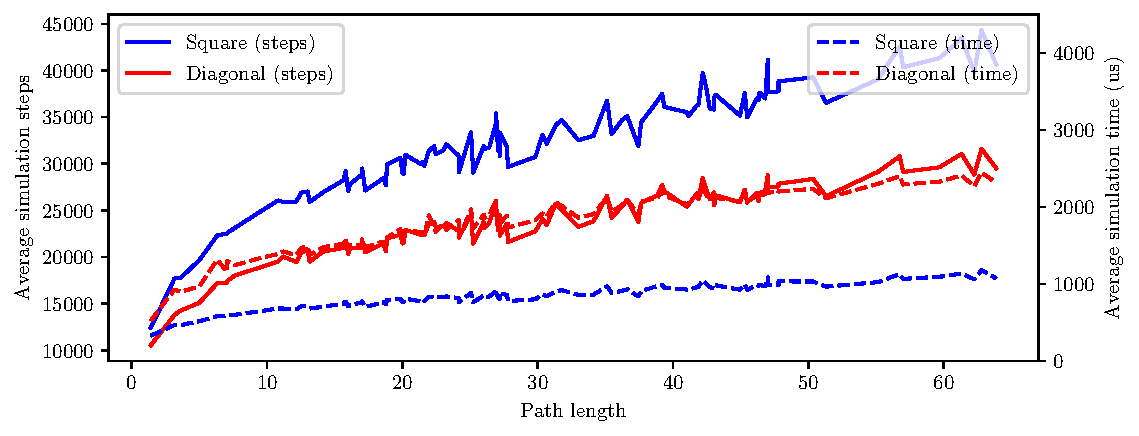
\includegraphics[width=14cm]{task1-compare}
    \caption[Comparison of multiple square and diagonal simulation steps]{Comparison of multiple square and diagonal simulation steps}
    \label{fig:task1-compare}
\end{figure}

Next, by plotting the ratio of the average number of steps taken by the square and diagonal movements we can establish a factor by which the diagonal movement is more efficient than the square movement.

\begin{figure}[ht]
    \centering
    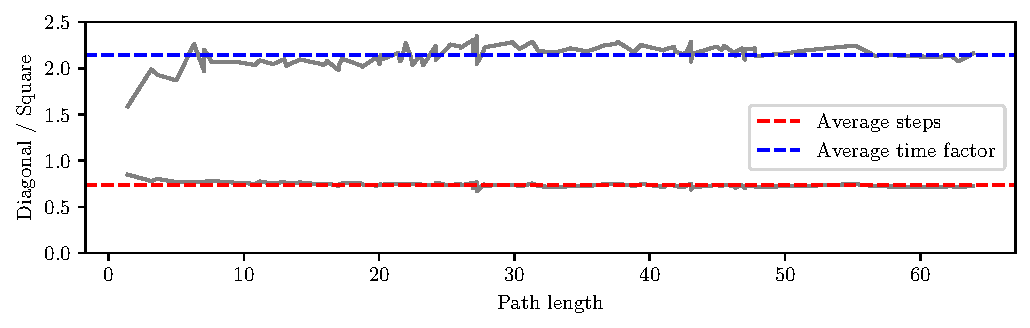
\includegraphics[width=14cm]{task1-factor-length}
    \caption[Comparison of multiple square and diagonal simulation steps (factor length)]{Comparison of multiple square and diagonal simulation steps (factor length)}
    \label{fig:task1-factor-length}
\end{figure}

The average factor for simulation steps is 0.7393 which is within the order of magnitude of the expected factor of 0.8284.

The discrepancy is ilkley due to additional factors such as the size of the grid and the number of iterations.
Non linear behaviour from the interactions at the edge of the grid to prevent the cells from moving off the grid.


The average factor for simulation time is 2.1436

Given the square movement is 0.3794 times faster than the diagonal movement,
and the diagonal movement takes 0.8284 times as many steps as the square movement,
the expected factor for simulation time is $0.3794 \times 0.8284 = 2.184$.

This is exceptionally close to the measured factor of 2.1436.

% Average steps factor: 0.7393451245144123
% Average time factor: 2.143568060901476

In conclusion, the diagonal movement is more efficient than the square movement in terms of the number of steps taken, but less efficient in terms of computational complexity. The computational complexity is significantly higher for the diagonal movement than the square movement, this overwhelms the number of steps taken. Hence, the square movement is more efficient than the diagonal movement overall.

\clearpage